\documentclass[a4paper,11pt,twoside]{article}
\usepackage[absolute,overlay]{textpos}
\usepackage[english]{babel} %% needed for refs not to get a "~"

\usepackage{lscape}
\usepackage{array}
\usepackage{geometry}
\geometry{verbose,a4paper,tmargin=23mm,bmargin=26mm,lmargin=30mm,rmargin=30mm}

\usepackage{setspace}
\singlespacing

\usepackage{graphicx}

\usepackage[latin1]{inputenc}
\usepackage{times}
\usepackage[T1]{fontenc}

\setcounter{secnumdepth}{5} %% paragraphs in toc
\setcounter{tocdepth}{5}


\usepackage{datetime} %% but I think I am not using it


\usepackage{tikz}
\usetikzlibrary{arrows,shapes,positioning}

\tikzset{
  % Define standard arrow tip
  >=stealth',
  % Define style for boxes
  punkt/.style={
    rectangle,
    rounded corners,
    draw=black, %very thick,
    %maximum width=6em,
    %text width=6.5em,
    minimum height=2em,
    text centered},
  punkt2/.style={
    rectangle,
    rounded corners,
    draw=black, %very thick,
    text width=2.35cm,
    %text width=6.5em,
    minimum height=2em,
    inner sep = 2pt,
    text centered},
  punkt3/.style={
    rectangle,
%    rounded corners,
    draw=black, %very thick,
%    text width=1.cm,
    %text width=6.5em,
    minimum height=2em,
    inner sep = 3pt,
    text centered},
  punkk/.style={
    rectangle,
    rounded corners=3mm,
    draw=black, %very thick,
    %text width=6.5em,
    minimum height=2em,
    text centered},
  ell1/.style={
    %ellipse,
    %draw = black, very thick,
    text width=1.7cm,
    inner sep = 0pt,
    text centered},
  % Define arrow style
  pil/.style={
    ->,
    thick,
    shorten <=2pt,
    shorten >=2pt,}
}




\usepackage{verbatim}
\usepackage{amsmath}
\usepackage[hyphens]{url}
\usepackage[pdftex]{hyperref}
%\usepackage{cite}

\usepackage{url}
\usepackage{xcolor}
\definecolor{light-gray}{gray}{0.72}
\newcommand{\cyan}[1]{{\textcolor {cyan} {#1}}}
\newcommand{\blu}[1]{{\textcolor {blue} {#1}}}
\newcommand{\Burl}[1]{\blu{\url{#1}}}
\newcommand{\Curl}[1]{{\small \url{#1}}} %% you need to scape #

\newcommand{\lgray}[1]{{\textcolor {light-gray} {#1}}}
\newcommand{\red}[1]{{\textcolor {red} {#1}}}
\newcommand{\green}[1]{{\textcolor {green} {#1}}}
\newcommand{\mg}[1]{{\textcolor {magenta} {#1}}}
\newcommand{\og}[1]{{\textcolor {PineGreen} {#1}}}
%\newcommand{\code}[1]{\texttt{\slshape\footnotesize #1}}
%\newcommand{\code}[1]{\texttt{\slshape #1}}
\newcommand{\code}[1]{\texttt{#1}}
\newcommand{\opage}[1]{\texttt{[p.\ #1]}}
\newcommand{\myverb}[1]{{\footnotesize\texttt {\textbf{#1}}}}
\newcommand{\Rnl}{\ +\qquad\ }
\newcommand{\Emph}[1]{\emph{\mg{#1}}}

\providecommand{\tabularnewline}{\\}

%\usepackage{harvard}
\usepackage[authoryear, round, sort]{natbib}
\bibliographystyle{myagsm} %%bbs and chicago does not show URLs 
%%bbs and chicago does not show URLs 

% /texmf/bibtex/bst/myagsm.bst
% and then do texhash

%% Algorithm2e needs to come after natbib!!
\usepackage[boxed,vlined,linesnumbered]{algorithm2e}


%% \usepackage{enumitem} %% not clear I need it
\usepackage{enumerate}

%% an ugly hack, because I cannot get anything else to work

% \newlist{exsection}{enumerate}{10}
% \setlist[exsection]{label*=\thesection.\arabic*.}

% \newlist{exsubsection}{enumerate}{10}
% \setlist[exsubsection]{label*=\thesubsection.\arabic*.}

% \newlist{exsubsubsection}{enumerate}{10}
% \setlist[exsubsubsection]{label*=\thesubsubsection.\arabic*.}


% \DeclareMathOperator*{\argmax}{arg\,max}
% \underset{x}{\operatorname{argmax}}



\title{Phylogenetic reconstruction. \\ \vspace*{25pt} \large  Class notes for BM-13, ``Bioinform�tica Avanzada y
Biolog�a de Sistemas'', 2014-2015.}

\author{Ram�n Diaz-Uriarte\\
              Dept. Bioqu�mica\\Universidad Aut�noma de Madrid \\ 
              \texttt{ramon.diaz@iib.uam.es} \\ 
              \Burl{http://ligarto.org/rdiaz} }

\date{\gitAuthorDate\ {\footnotesize (Release\gitRels: Rev:
    \gitAbbrevHash)}}

%\date{}

%\date{\ddmmyyyydate \today} %needs datetime package
%% \date{\the\year-\the\month-\the\day}


\makeindex


\begin{document}

\maketitle
\vspace{-0.5cm}


\tableofcontents
\clearpage


\section{Pedagogical and scientific objectives of this module}
\begin{itemize}
\item Understand the major approaches to inferring phylogenies.
\item Gain further understanding of maximum likelihood and Bayesian approaches.
\item Be aware of some recent challenges and difficulties in phylogenetic
  inference with high-throughput data.
\end{itemize}





\section{Readings}



Start reading the chapter from \cite{Higgs-Attwood}. You can skip the
section about quartet-puzzling and go quickly over section 8.8.4 (the
example). 

You can take a look at the slides ``Phylog-diapos-licenciatura.pdf''. I
use them for the Phylogenies part of the Bioinformatics classes for the
bachelor's degree (4� Bioqu�mica). This is at less technical level than
covered in BM-13, of course, but we deal with issues we will not cover
here. If all of this seems too hard, I might use them to lecture with them
on the first day.

% You can see some further details and worked examples about UPGMA and NJ
% in the pages from \cite{Haubold2006}. Note error in UPGMA; and typo in
% Figure 8. 15.

When reading about ML (maximum likelihood) you might also want to look at
the two pages from \cite{Felsenstein2004}. This is an extremely clear
explanation of what is being done.


Then, read the pages from \cite{Durbin1998}. The first part gives further
details about number of trees, etc. No need to memorize it, but there is
one exercise where this is used. There are also some additional details
about UPGMA and NJ. The second part deals with probabilistic
models. Section 8.2 is there only as additional reference material, but
you can skip it. Pages 197--202 look hard, but they walk step-by-step over
likelihood. This might help you understand what likelihood is about.  The
rest is additional reference material.

% You should also understand the general ideas behind reversibility and
% independence of the root position.


Finally, read the paper by \cite{Blair2010}. We will discuss this in
class. Note that the differences between species and gene trees can be
crucial, but are not emphasized enough in \cite{Higgs-Attwood}. 


I have also uploaded the paper by \cite{Maddison1997}. This is just
provided as reference material, and you can skip it, but it gives nice and
thorough explanations of what the ``deep coalescence'' or ``gene sorting''
problems are about, and thus could help to make sense of some of the
issues raised by \cite{Blair2010}. You might want to read just pages
525--527 in \cite{Maddison1997}.


\section{Further notes}
\label{sec:further-notes}



\subsection{Number of substitutions and evolutionary time}
\label{distances-time}

What we care about, when reconstruction evolutionary relationships, are
distances that reflect amount of change. This is hinted at in p.~162 of
\cite{Higgs-Attwood}, and this is what section 8.2 of \cite{Durbin1998} is
about. Chapter 4 of \cite{Higgs-Attwood} is devoted fully to this topic.

To summarize, in a few lines: simply counting the number of substitutions
between two sequences will underestimate the true number of changes (think
about multiple substitutions).  With a model such as the one of Jukes and
Cantor we get a relationship like the one in Figure \ref{JC-time}. (Note:
you can relate the 0.75 in the abscisas to one of the exercises we did in
the probability part; which one?)


 \begin{figure}[h!]
\begin{center}
   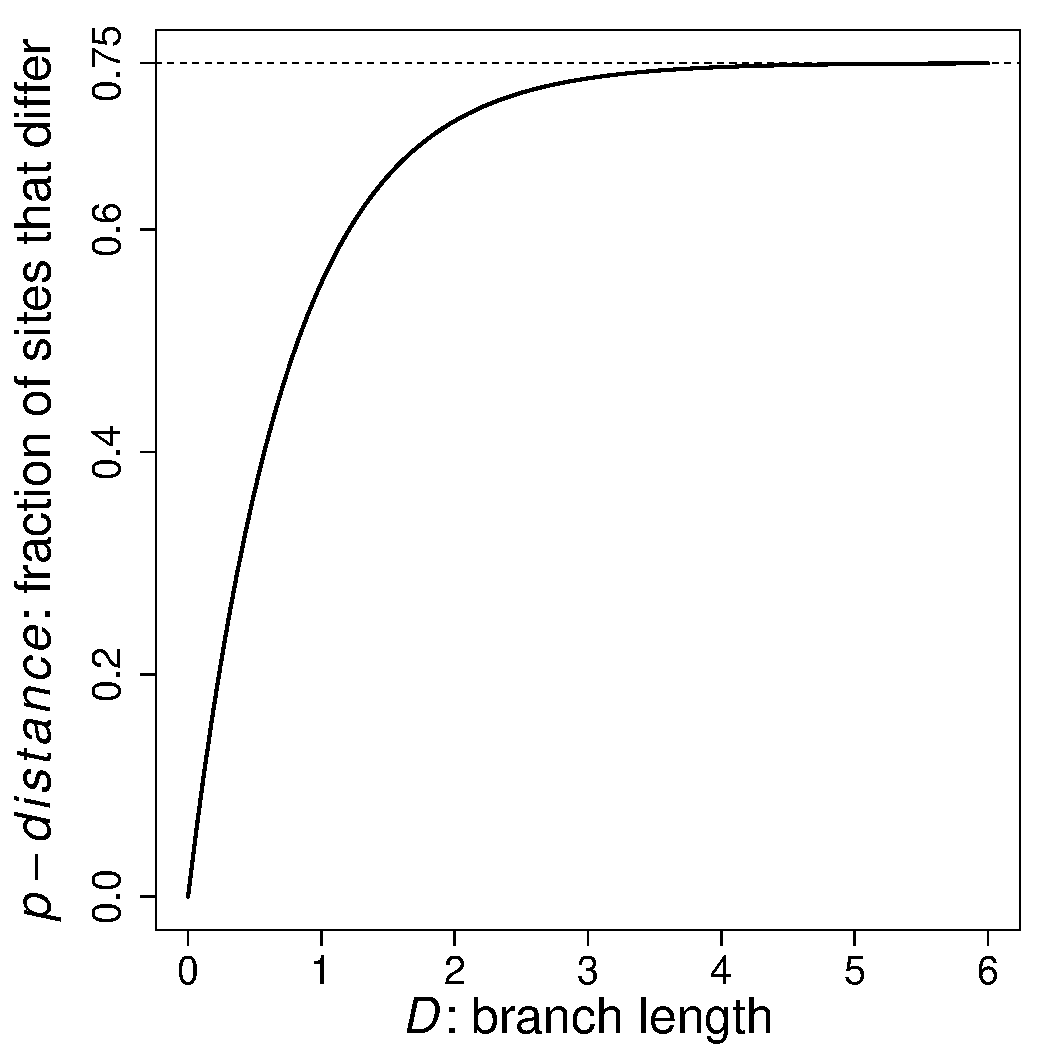
\includegraphics[width=8.1cm,keepaspectratio]{JC2.pdf}
\end{center}
   \caption{\label{JC-time} Fraction of sites that differ vs.\ true
     evolutionary distance, for the Jukes-Cantor model. 
$D = -\frac{3}{4} \ln (1 - \frac{4p}{3})$, where $p$ is the fraction of sites that
     differ and $D$ is the true number of changes (nucleotide
     substitutions per site).  Therefore, $p = \frac{3}{4} (1 - \exp^{-\frac{4D}{3}})$}

%% And time? If we knew \alpha, it would be K/(3\alpha)
% (and ``time'' would be $3 \alpha K$, where
  % $\alpha$ is the transition rate)

 \end{figure}
%% see notes of sys biol for creating JC2.pdf

% pdf(file = "JC.pdf")
% par(cex.lab = 1.6)
% par(mar = c(4, 5, 1, 1))
% par(oma = c(0, 0.2, 0, 0))
% jc <- function(x) -(3/4) * log(1 - (4/3) * x)
% curve(jc, 0, 0.745, xlab = expression(paste(italic(f), ": fraction of sites that differ")), 
% ylab = expression(paste(italic(K), ": true number of changes")), xlim = c(0, 0.76))
% axis(1, at = 0.75, lab = c(0.75))
% dev.off()



Beware: this is a \textbf{way too short} summary. For instance, we are not
discussing a common modification of J-C which is to add variability to
rates. We are also not discussing other models. The main point here is to
understand:
\begin{itemize}
\item Observed substitutions underestimate true number of changes.
\item Estimating the true number of changes requires a model.
\item We should NOT use uncorrected distances to build evolutionary
  trees. There is a nice example of the consequences in
  \citet[][p.~158--159]{Felsenstein2004}.
\end{itemize}

\subsection{Numbers of trees and nodes}
\label{sec:numbers-trees-nodes}

Pages 163 and 164 of \citet{Durbin1998} show how one derives the number of
trees, nodes, and edges (branches). You do not need to memorize the
expressions, but you have them here for reference.





\subsection{The four-point condition}
The four-point condition can be used as a test for additivity. It is
explained in p.~ 172 of \citet{Durbin1998} though not referred to
explicitly in \citet{Higgs-Attwood}.



\section{EXERCISES:  Phylogenies}
\label{exerc-hmms}

\begin{enumerate}

\item \label{bm13-filog1}Number of trees, number of branches, distances. % basado en Haubol, 8.1, 8.2
      
This is a multiple alignment of four different species:


\begin{verbatim}
A   GGTACGCTCT
B   CGATCCATCT
C   CCAAGGCTCA
D   GGAAGGCTTT

\end{verbatim}

%% Eh! Two positions are informative. Delete/change the first or the fifth
%% column FIXME zz Nope, leave it.

\begin{enumerate}
\item How many rooted trees could you build?
\item How many unrooted trees?
\item How many internal nodes would there be?
\item How many branches (edges), both internal and external?
\item Compute the distance between the four species as number of
  substitutions.
\item Compute the distances ($K$ in the figure above) $d_{AB}, d_{AC},
  d_{BD}$ using the Jukes-Cantor model.
\end{enumerate}


\item UPGMA, phylogenies, and microarrays.

When reconstructing phylogenies we use data
that (are supposed to) reflect evolutionary distances. With microarray
data we use a different set of distances. Do you understand the
similarities and differences? What is common and what is not in the two
scenarios? 



\item \label{ex81-ha} Exercise 8.1 in \citet{Higgs-Attwood}. The three parts a), b),
  c). 

  But note that \textbf{figure b) is wrong!} Nodes ``C'' and ``D'' should be
  exchanged (so node D has to be the closest relative to A, and node C has
  to be the closest relative to B)

%% If not additive: either NJ or Fitch Margoliash and related.


  Now, use the NJ algorithm, to find the phylogeny (yes, we already know it,
  but we want to practice with the algorithm). 

\item With the data from exercise \ref{ex81-ha}, using only the original
  distance (not any transformations with the JK model), verify the
  four-point condition.


\item Using the data in \ref{bm13-filog1} reconstruct the phylogeny of
  those four species using:

  \begin{enumerate}
  \item UPGMA. Is the phylogeny rooted? Are distances ultrametric? When
    you do the reconstruction, use \textbf{the original data} (so in this
    case do not transform using Jukes-Cantor ---we do this for simplicity;
    using a model should almost always be done for real).
  % \item NJ. Is the phylogeny rooted? Are distances additive?
  \item Maximum parsimony. (No, yo do not need to use sophisticated
    algorithms; just look carefully at the 10 characters to see which are
    informative). Use a rooted tree. 
  \end{enumerate}

%% FIXME: OJO: que en upgma usen datos originales, y ojo con el de
%% parsimonia. Comparar a�os 2012 y 2013, porque en 2013 fue un jaleo


 % Haub. 8.3, 8.7. 
 %% Ojo, corrijo los datos, porque en original la posicion 7 no estaba
 %% bien.
%% I modifico los datos moviendo las columnas. Ahora  la 7 es la 5.



\item Reconstructing phylogenies by maximum likelihood.

  Box 8.2 in \citet[][p.~ 174]{Higgs-Attwood} and pp.~197--202 of
  \cite{Durbin1998} both explain maximum likelihood.  The two pages from
  Felsenstein do the same thing. However, they explain it in slightly
  different ways. Make sure you understand them. One might be easier to
  follow first than the other, but they are all saying the same thing. For
  instance, equation 8.10 in \cite{Durbin1998} is the same as equation
  16.11 in Felsenstein, and the same to equation 8.11 (with eq. 8.10 and
  8.9 and 8.8 plugged in) in \cite{Higgs-Attwood}.



\item Read the paper by \cite{Blair2010}.

  What are the main challenges in phylogenetic reconstruction with
  high-throughput data? Where do you think Bayesian inference would be
  more advantageous? Where have we seen before the usage of reversible
  jump? Could your current work be affected by the difference between
  species trees and gene trees?


%% Yo: revisare linage sorting y coalescence

\item You should be able to answer and argue the following questions:

  \begin{enumerate}
  \item Of the methods shown, which one is (virtually) never to be used
    ``for real''?
  \item Among the other approaches, which one you think is ``best'' and
    why?

  \item You have a huge data set (many species, lots and lots of
    characters; for instance, very long sequences). What would you use to
    reconstruct the phylogeny? Would you be able to use neighbor joining
    with these data? And maximum likelihood?

  \item You have new type of data, for which no good evolutionary model
    has been developed yet. How could you try to reconstruct the
    phylogeny? What steps could you follow?

  \item Bayesian methods for phylogenetic inference do use the likelihood,
    but can be much faster than pure maximum likelihood approaches. What
    is the trick?

  \item Are there any features of Bayesian approaches that you could find
    troublesome?

  \item Bootstrapping can help (or not) assess the evolutionary model;
    bootstraping can be used (or not) if the rate of substitution varies
    over sites; bootstrapping can be used (or not) with maximum likelihood
    methods.
  \end{enumerate}

\end{enumerate}


\section{A few bibliographic notes}

Probably the (so far) definitive ``bible'' about phylogenetic inference is
\cite{Felsenstein2004}. A volume that includes some more recent work, as
well as practical computer exercises, is
\cite{Lemey2009}. \cite{Durbin1998} and \cite{Higgs-Attwood} also have
great chapters on phylogenetic inference.  \cite{Graur2010} has a chapter
devoted to phylogenetic inference, and several nice and detailed examples
of the use of molecular phylogenies ``in real life''. % \cite{Haubold2006}
% also contain chapters on phylogenetic inference. 
For those who want a very
practical book, with guided computer usage, one of the best
recommendations is \cite{Hall2011}, now in its fourth
edition. Phylogenetic inference is a fertile field, and there are many
other recent monographical references.% Other recent, more technical
% books, include \cite{Yang2006} and \cite{Gascuel2005}.


%% Papers on reconstruction of ancestral states.



\bibliography{library}


\end{document}



*** Phylogenies
    - [ ] Deonier
    - [ ] Ewens and Grant
    - [ ] Aluru, p. 516 (Tarnow chapter)
    - [ ] Haubold and Wiehe
    - [ ] Neapolitan,   Probabilistic methods for bioinfo, cap. 11
    - [ ] Heath and Ramkrishnan, "Problem solving handbook"   p. 101
    - [ ] Yang??







%% Este puede tener cosas interesantes, ej. filogenia (p. 110)
%% Problem Solving Handbook in Computational Biology and Bioinformatics





%% very clean run:
%% rm *.idx; rm *.toc; rm *.out; rm *.blg; rm *.log; rm *.aux; rm *.dvi; rm *.bbl; texi2pdf algorithms-class-notes.tex

%%% Local Variables:
%%%   mode: latex
%%%   mode: flyspell
%%%   coding: iso-8859-15
%%% End:



